\section{Dreidimensionales Punktdiagramm}

Falls Datensätze mit einer unabhängigen und zwei abhängigen Variablen dargestellt werden sollen, kann ein dreidimensionales Punktdiagramm verwendet werden.

Beispiele für Datensätze, die in dreidimensionalen Punktdiagrammen dargestellt werden können:

\begin{itemize}
	\item Zwei Attribute im Laufe der Zeit, zum Beispiel BIP und Arbeitsplätze eines Landes
	\item Drei Attribute, die in einem bestimmten Verhältnis zueinander stehen. Zum Beispiel Geschwindigkeit, Luftwiderstand, Oberfläche
\end{itemize}

Es wurde entschieden, eine weitere Applikation zu entwickeln, die einen Datensatz mit einer unabhängigen und zwei abhängigen Variablen in einer 3D-Applikation anzeigt. Dazu wurden Daten der World Bank \cite{worldbank} zur Bevölkerung und Arbeitsplätzen der Schweiz im Verlauf der Zeit verwendet.

\subsection{Applikation}

\begin{figure}[H]
	\centering
	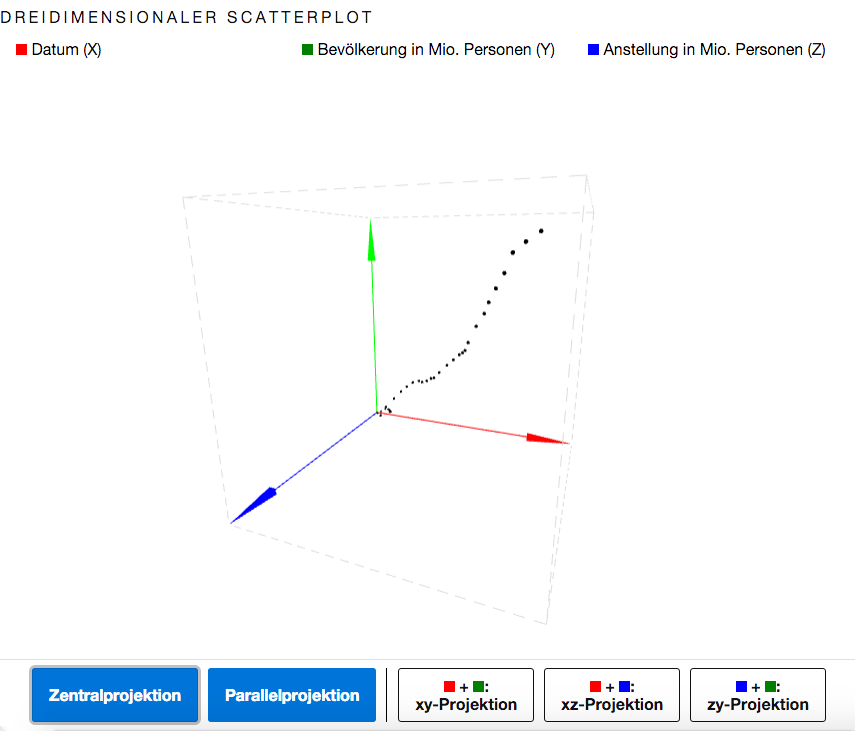
\includegraphics[width=\linewidth]{images/3d}
	\caption{Oberfläche der Applikation (dreidimensionales Punktdiagramm), perspektivische Projektion}
	\label{fig:3d}
\end{figure}

Abbildung \ref{fig:3d} zeigt die Oberfläche der entwickelten Applikation. Der Name des Tests in der Applikation lautet \texttt{3d}. Die Programmbibliothek \textit{three.js} \cite{threejs} wurde verwendet; three.js ermöglicht die Entwicklung von 3D-Applikationen mit JavaScript im Browser.

\textbf{Achsen.} Als Achsen wurden verschiedenfarbige Pfeile (Abbildung \ref{fig:vectors}) mit Richtungsvektoren $\vec{a}_x$, $\vec{a}_y$, und $\vec{a}_z$ erstellt.

\begin{figure}[H]
	\centering
	$\vec{a}_x=\begin{pmatrix} 1 \\ 0 \\ 0 \end{pmatrix}$ (rot)\qquad
	$\vec{a}_y=\begin{pmatrix} 0 \\ 1 \\ 0 \end{pmatrix}$ (grün)\qquad
	$\vec{a}_z=\begin{pmatrix} 0 \\ 0 \\ 1 \end{pmatrix}$ (blau)\qquad
	\caption{Die Richtungsvektoren der Achsen im dreidimensionalen Punktdiagramm.}
	\label{fig:vectors}
\end{figure}

Die Beschriftung und Farben der Achsen werden über dem Diagramm angezeigt. Die erste Beschriftung (rot) steht für die unabhängige Variable, die zweite und dritte Beschriftung (grün und blau) für die abhängigen Variablen.

\textbf{Punkte.} Die Datenpunkte wurden an den drei Achsen abgetragen und als schwarze Kugeln im Raum abgebildet.

\textbf{Würfel.} Ein Würfel wurde mit gestrichelten grauen Linien um das Diagramm dargestellt. Es soll dem Benutzer helfen, sich in dem dreidimensionalen Raum zu orientieren.

\textbf{Rotation.} Das dreidimensionale Punktdiagramm ist mit der Maus rotierbar. Die Kamera bleibt während der Rotation stets auf die Mitte des Diagramms gerichtet. Die Rotation ermöglicht eine bessere Erkundung des Datensatzes und bietet die Ansicht aus verschiedenen Winkeln dar.

Eine Funktion für das Zoomen wurde nicht implementiert, weil sie sich als kontraproduktiv herausstellte: Die Orientierung des Benutzers geht schnell verloren, zum Beispiel wenn zu weit herausgezoomt wird, sodass das Diagramm nicht mehr sichtbar ist, oder wenn sich die Kamera innerhalb der Punktewolke befindet.

\subsection{Reduktion auf zweidimensionale Punktdiagramme durch Projektion}

Eine besondere Erkenntnis bei der Entwicklung dieser Applikation ist das Erkennen des Potentials von orthographischen Projektionen innerhalb des dreidimensionalen Punktdiagramms.

Das Punktdiagramm kann durch Verschieben der Kamera und Verwendung der orthographischen Projektion auf ein zweidimensionales Punktdiagramm reduziert werden.

Zum Beispiel führt die Projektion der zy-Fläche zur Darstellung eines zweidimensionalen Punktdiagramms: Die \textit{neue Abszisse}\footnote{Mit dem Begriff "`\textit{neue Abszisse}"' ist die Abszisse des neu dargestellten, zweidimensionalen Punktdiagramms gemeint.} ist die y-Achse, die \textit{neue Ordinate}\footnote{Mit dem Begriff "`\textit{neue Ordinate}"' ist ebenfalls die Ordinate des neu dargestellten, zweidimensionalen Punktdiagramms gemeint.} die z-Achse. Der Effekt kann in diesem Beispiel erzielt werden, wenn die Kamera auf negativer x-Achsen-Position, halber y-Achsen-Position und halber z-Achsen-Position ist und in die Richtung der Mitte des Diagramms ausgerichtet ist.

Abbildung \ref{fig:3dmath} erklärt Funktionsweise der Projektion: Sei $S$ der Schnittpunkt der Abszissenachse (x), Ordinatenachse (y) und Applikatenachse (z), $M$ der Mittelpunkt des Diagramms und $P_{\text{xy}}$, $P_{\text{xz}}$, $P_{\text{zy}}$ die Position der Kamera für die entsprechende Projektion:

\begin{figure}[H]
$$S = (0|0|0)$$

$$M = (\frac{a}{2} | \frac{a}{2} | \frac{a}{2})$$

$$P_{\text{xy}} = (\frac{a}{2} | \frac{a}{2}| a + a)$$

$$P_{\text{xz}} = (\frac{a}{2} | -a | \frac{a}{2})$$

$$P_{\text{zy}} = (-a | \frac{a}{2}| \frac{a}{2})$$

\caption{Positionen der Kamera für Projektionen im dreidimensionalen Punktdiagramm.}
\label{fig:3dmath}
\end{figure}

Somit stehen je zwei Achsen bei $P_{\text{xy}}$, $P_{\text{xz}}$ oder $P_{\text{zy}}$ senkrecht, die verbleibende Achse steht parallel zur Kamerarichtung; in Abbildung \ref{fig:3dtable} werden die neue Abszisse und Ordinate des projizierten zweidimensionalen Punktdiagramms und die Kamerarichtung nach Projektion aufgelistet.

\begin{figure}[H]
	\centering
	\begin{tabular}{ | m{0.15\linewidth} | m{0.2\linewidth} |m{0.2\linewidth} | m{0.3\linewidth} |}
		\hline
		\textbf{Projektion} & \textbf{neue Abszisse} & \textbf{neue Ordinate} & \textbf{Kamerarichtung}\\ \hline
		xy & Abszissenachse (x) & Ordinatenachse (y) & Entgegen der Applikatenachse (z) \\ \hline
		xz & Abszissenachse (x) & Applikatenachse (z) & In Richtung Ordinatenachse (y)\\ \hline
		zy & Applikatenachse (z) & Ordinatenachse (y) & In Richtung Abzissenachse (x) \\ \hline
	\end{tabular}
	\caption{Beschreibung des projizierten zweidimensionalen Punktdiagramms nach Projektion}
	\label{fig:3dtable}
\end{figure}

In Abbildung \ref{fig:projections} wird die Projektion der xz-Ebene angezeigt. Bei dem linken Beispiel wird die \textit{perspektivische Projektion} verwendet. Die perspektivische Projektion wird in den meisten 3D-Applikationen verwendet. Die Geraden verlaufen durch einen festen Punkt. Das Auge verwendet ebenfalls die perspektivische Projektion: Strahlen werden so auf der Netzhaut abgebildet.

Die perspektivische Projektion hat den Nachteil, dass sie Objekte verzerrt, je nachdem, wie weit sie entfernt sind. Sie ist für unsere Zwecke (der Reduktion des dreidimensionalen Punktdiagramm auf ein zweidimensionales) nicht geeignet.

Bei der orthographischen Projektion hingegen werden Punkte auf einer Ebene abgebildet und somit nicht verzerrt, falls sie weiter entfernt von der Projektionsfläche liegen. Beim rechten Beispiel in Abbildung \ref{fig:projections} ist somit das dreidimensionale Punktdiagramm auf ein zweidimensionales Punktdiagramm reduziert worden.

\begin{figure}[!htbp]
	\centering
	\begin{minipage}{.45\textwidth}
		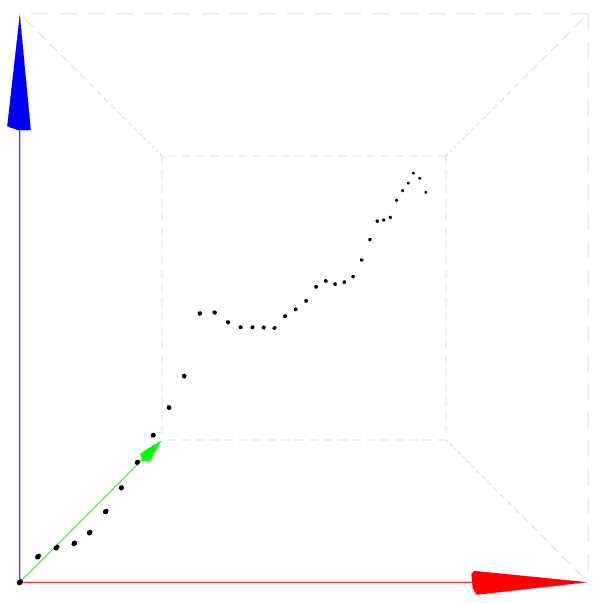
\includegraphics[width=\linewidth]{images/persp}
	\end{minipage}
	\begin{minipage}{.45\textwidth}
		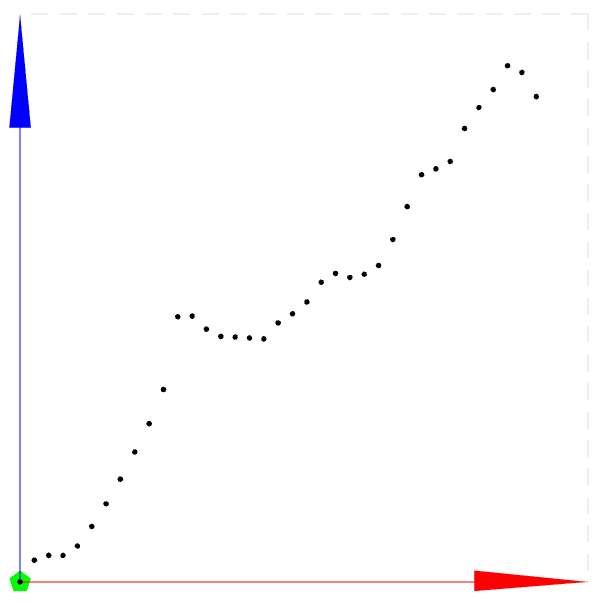
\includegraphics[width=\linewidth]{images/ortho}
	\end{minipage}
	\caption[Projektion der xz-Ebene]{Projektion der XZ-Ebene. Links: Perspektivische Projektion. Rechts: Orthographische Projektion.}
	\label{fig:projections}
\end{figure}

Es ist in der Applikation möglich, zwischen der perspektivischen und orthographischen Projektion, sowie zwischen der xy-, xz- und zy-Projektion umzuschalten. Der Benutzer kann sich so besser mit dem Datensatz auseinandersetzen, indem er einfach zwischen dreidimensionalem und zweidimensionalem Punktdiagramm navigieren kann.

Damit der Benutzer die Orientierung behält, wird die Kamerabewegung zwischen $P_{\text{xy}}$, $P_{\text{xz}}$ und $P_{\text{zy}}$ animiert. Dazu wird die JavaScript-Bibliothek \textit{tween.js} \cite{tween} verwendet.